\documentclass[12pt, a4paper]{report}

% ==============================================================================
% KMOU OceanX International Summer School 2026 - Project Report
% ==============================================================================

\usepackage{graphicx}
\usepackage{amsmath, amssymb}
\usepackage{geometry}
\usepackage{pgfgantt}
\usepackage{setspace}
\usepackage{cite}
\usepackage{hyperref}
\usepackage{titlesec}
\usepackage{caption}
\usepackage{listings}
\usepackage{booktabs}
\usepackage{xcolor}
\usepackage{tikz}
\usepackage{pdflscape}
\usepackage{array}
\usepackage{tabularx}
\usepackage{longtable}
\usepackage{float}
\usepackage{url}

\usetikzlibrary{shapes.geometric, arrows, positioning}

% TikZ styles for architecture diagrams.
\tikzstyle{startstop} = [rectangle, rounded corners, minimum width=3cm, minimum height=1cm, text centered, draw=blue!60!black, fill=blue!5, thick]
\tikzstyle{process} = [rectangle, rounded corners, minimum width=3cm, minimum height=1cm, text centered, draw=blue!60!black, fill=blue!5, thick]
\tikzstyle{decision} = [diamond, aspect=2, minimum width=3cm, minimum height=1cm, text centered, draw=blue!60!black, fill=blue!5, thick]
\tikzstyle{arrow} = [thick,->,>=stealth, draw=blue!60!black]

\lstset{
  basicstyle=\ttfamily\small,
  breaklines=true,
  frame=single,
  keywordstyle=\color{blue},
  stringstyle=\color{red},
  commentstyle=\color{green!50!black},
  showstringspaces=false,
  numbers=left,
  numberstyle=\tiny\color{gray},
  captionpos=b
}

\geometry{
    top=2cm,
    bottom=2.5cm,
    left=1in,
    right=1in
}
\onehalfspacing

\hypersetup{
    colorlinks=true,
    linkcolor=black,
    filecolor=magenta,
    urlcolor=black,
    citecolor=black,
    plainpages=false
}

\captionsetup[table]{justification=centering,singlelinecheck=false}

\begin{document}

\title{Development of an OpenCPN EEXI-CII Operational Awareness Plugin with Real-Time CII Monitoring}
\author{Nahadi Farid}
\date{July 2026}

% ==============================================================================
% TITLE PAGE
% ==============================================================================
\hypersetup{pageanchor=false}
\begin{titlepage}
\thispagestyle{empty}
\begin{center}

{\setstretch{1.0}
\vspace*{0.7cm}

{\Large \textbf{KOREA MARITIME \& OCEAN UNIVERSITY}}\\[0.3cm]
{\large \textbf{KMOU OceanX International Summer School 2026}}\\[0.3cm]
{\normalsize Project Report}\\[1.0cm]

\hrule
\vspace{0.45cm}

{\Large \textbf{DEVELOPMENT OF AN OPENCPN}}\\[0.12cm]
{\Large \textbf{EEXI-CII OPERATIONAL AWARENESS}}\\[0.12cm]
{\Large \textbf{PLUGIN WITH REAL-TIME CII MONITORING}}

\vspace{0.45cm}
\hrule
\vspace{1.0cm}

{\normalsize Prepared by}\\[0.25cm]
{\large \textbf{NAHADI FARID}}\\[0.1cm]
{\normalsize Marine Engineering Participant}\\[0.1cm]
{\normalsize ENM241-0143/2021}\\[0.8cm]

{\normalsize Project Area}\\[0.2cm]
{\large \textbf{Maritime Decarbonisation, Open-Source Navigation, and Ship Energy Efficiency}}\\[0.8cm]

{\normalsize Submitted for}\\[0.2cm]
{\large \textbf{KMOU OceanX International Summer School 2026}}\\[0.2cm]
{\normalsize Korea Maritime \& Ocean University, Busan, South Korea}\\[0.8cm]

{\normalsize Project Version}\\[0.2cm]
{\large \textbf{Prototype v0.1.0}}\\

\vfill

{\footnotesize This report documents an operational-awareness software prototype.}\\
{\footnotesize It is not a class-society validation document and is not intended for official IMO submissions.}\\[0.2cm]
{\footnotesize July 2026}
}

\end{center}
\end{titlepage}
\hypersetup{pageanchor=true}

% ==============================================================================
% FRONT MATTER
% ==============================================================================
\pagenumbering{roman}

\section*{PROJECT INFORMATION}
\addcontentsline{toc}{section}{Project Information}

\begin{tabularx}{\textwidth}{lX}
\toprule
\textbf{Item} & \textbf{Description} \\
\midrule
Host programme & KMOU OceanX International Summer School 2026 \cite{kmouOceanX2026} \\
Host institution & Korea Maritime \& Ocean University (KMOU), Busan, South Korea \\
Project title & Development of an OpenCPN EEXI-CII Operational Awareness Plugin with Real-Time CII Monitoring \\
Participant & Nahadi Farid \\
Primary deliverable & C++ OpenCPN plugin prototype named \texttt{eexi\_cii\_pi} \\
Prototype status & Core/test build passing; OpenCPN plugin wrapper, setup dialog, dashboard, JSON persistence, diagnostics, CSV export, demo feed, and packaging script present in the repository \\
Validation boundary & Automated and synthetic replay validation only; no class-society, statutory, or real-vessel fuel-flow validation has been completed \\
\bottomrule
\end{tabularx}

\newpage

\chapter*{Acknowledgements}
\addcontentsline{toc}{section}{Acknowledgements}

The author acknowledges the KMOU OceanX International Summer School 2026 organisers for providing a maritime innovation context for this work, the OpenCPN community for maintaining an open navigation platform, and the International Maritime Organization for publishing the regulatory framework that motivates transparent emissions-awareness tooling. Appreciation is also extended to mentors, lecturers, and peers who supported the development and review of this prototype.

\newpage

\chapter*{Abstract}
\addcontentsline{toc}{section}{Abstract}

This project report documents the design, implementation, and validation status of an open-source OpenCPN plugin prototype for ship emissions operational awareness. The implemented software focuses on real-time Carbon Intensity Indicator (CII) monitoring for the vessel running OpenCPN. It parses own-ship NMEA 0183 RMC sentences, validates checksums and data status, estimates main-engine fuel use and carbon dioxide emissions using the Admiralty Coefficient method, accumulates distance with a Haversine geodesic calculation, and computes running AER or cgDIST values against source-tagged IMO CII reference data for 2023--2026. The prototype includes a wxWidgets setup dialog, dashboard, diagnostics view, JSON persistence, annual and voyage CSV export, a synthetic NMEA demo feed, and an OpenCPN plugin-manager packaging script. The EEXI portion is represented as project context and setup data fields; a full statutory EEXI pass/fail calculator is not implemented in this version. Automated validation on the current repository passed all six CTest entries, including domain, parser, accumulator, replay, and packaging checks. The synthetic replay fixture produced 180.121 nm of distance, 8.343 tonnes of estimated CO$_2$, an AER of 0.579 gCO$_2$/(dwt-nm), and an A rating for the configured bulk-carrier test profile. The prototype is therefore suitable as a demonstrable summer-school project and research tool, but it remains an operational-awareness system only and must not be used as a substitute for official DCS, SEEMP, EEXI, or CII regulatory verification.

\tableofcontents
\listoffigures
\listoftables

\clearpage

\section*{LIST OF ABBREVIATIONS AND SYMBOLS}
\addcontentsline{toc}{section}{List of Abbreviations and Symbols}

\subsection*{Abbreviations}
\begin{tabular}{ll}
\textbf{AER} & Annual Efficiency Ratio \\
\textbf{API} & Application Programming Interface \\
\textbf{CII} & Carbon Intensity Indicator \\
\textbf{CSV} & Comma-Separated Values \\
\textbf{DCS} & IMO Data Collection System \\
\textbf{DWT} & Deadweight Tonnage \\
\textbf{EEDI} & Energy Efficiency Design Index \\
\textbf{EEXI} & Energy Efficiency Existing Ship Index \\
\textbf{GHG} & Greenhouse Gas \\
\textbf{GNSS} & Global Navigation Satellite System \\
\textbf{GPS} & Global Positioning System \\
\textbf{GT} & Gross Tonnage \\
\textbf{IMO} & International Maritime Organization \\
\textbf{JSON} & JavaScript Object Notation \\
\textbf{KMOU} & Korea Maritime \& Ocean University \\
\textbf{MARPOL} & International Convention for the Prevention of Pollution from Ships \\
\textbf{NMEA} & National Marine Electronics Association \\
\textbf{RMC} & Recommended Minimum Specific GPS/Transit Data \\
\textbf{SEEMP} & Ship Energy Efficiency Management Plan \\
\textbf{SFOC} & Specific Fuel Oil Consumption \\
\textbf{SOG} & Speed Over Ground \\
\textbf{UDP} & User Datagram Protocol \\
\textbf{UTC} & Coordinated Universal Time \\
\end{tabular}

\vspace{1cm}

\subsection*{Symbols}
\begin{tabular}{ll}
$\Delta$ & Vessel displacement (tonnes) \\
$C$ & Admiralty Coefficient \\
$C_F$ & Fuel-to-CO$_2$ conversion factor (t-CO$_2$/t-fuel) \\
$D_t$ & Distance sailed (nautical miles) \\
$d_1, d_2, d_3, d_4$ & IMO CII rating boundary vectors \\
$P$ & Estimated shaft power (kW) \\
$V$ & Vessel speed (knots) \\
$Z$ & Annual CII reduction factor (\%) \\
\end{tabular}

\newpage

\clearpage
\pagenumbering{arabic}

\chapter{Introduction}
\label{chap:introduction}

\section{Summer School Project Context}
This report has been prepared as a project report for the KMOU OceanX International Summer School 2026. The programme was announced by Korea Maritime \& Ocean University through its official English notice board in April 2026 \cite{kmouOceanX2026}. The project aligns with the summer school's ocean-technology theme by combining maritime decarbonisation, open-source navigation software, and practical ship-energy monitoring.

The software artefact developed for this project is an OpenCPN plugin prototype named \texttt{eexi\_cii\_pi}. OpenCPN is a free and open-source chartplotter and marine GPS navigation platform used on Windows, macOS, Linux, Raspberry Pi, and Android \cite{opencpnOfficial2026}. The project therefore uses an existing navigation environment rather than creating a standalone emissions dashboard.

\section{Background and Motivation}
The decarbonisation of maritime transport has become a central regulatory and engineering concern. The Fourth IMO GHG Study reported that total shipping greenhouse gas emissions, including international, domestic, and fishing activity, increased from 977 million tonnes CO$_2$e in 2012 to 1,076 million tonnes CO$_2$e in 2018, while the sector's share of global anthropogenic emissions rose from 2.76\% to 2.89\% over the same period \cite{imoFourthGhg2020}. The same study found that international shipping carbon intensity had improved relative to 2008, but that total emissions continued to place pressure on the sector's climate pathway.

The IMO's 2023 Strategy on Reduction of GHG Emissions from Ships sets the long-term ambition of reaching net-zero GHG emissions from international shipping by or around 2050 and includes a target to reduce average international shipping carbon intensity by at least 40\% by 2030 compared with 2008 \cite{imoGhgStrategy2026}. The short-term regulatory measures supporting this transition include the Energy Efficiency Existing Ship Index (EEXI) and the annual operational Carbon Intensity Indicator (CII). IMO states that MARPOL Annex VI amendments entered into force on 1 November 2022, with EEXI and CII requirements taking effect on 1 January 2023 \cite{imoEexiCiiFaq2026}.

CII is especially operational because it turns fuel consumption, distance sailed, and ship capacity into an annual A--E rating. A ship rated D for three consecutive years, or E for one year, must submit a corrective action plan showing how it will achieve a C rating or better \cite{imoEexiCiiFaq2026}. This makes mid-year awareness important: if a ship only analyses its CII performance at the end of the reporting year, many operational options have already passed.

\section{Problem Statement}
Many compliance workflows remain retrospective. Operators may gather fuel and distance data for annual reporting, but masters and engineers often lack a live, navigation-integrated view of how present speed and voyage behaviour affect the vessel's year-to-date CII trajectory. Commercial platforms exist, but they may require proprietary systems, subscription models, satellite connectivity, or direct integration with fuel-flow sensors.

This creates a practical access gap for smaller operators, research users, training environments, and developing maritime contexts. A lightweight OpenCPN plugin can demonstrate how live own-ship navigation data can be transformed into operational emissions awareness without requiring additional shipboard instrumentation. The project does not attempt to replace statutory verification. Instead, it explores how open-source software can make CII concepts visible during navigation and training.

\section{Project Aim and Objectives}
The aim of this project is to design, implement, and validate a demonstrable OpenCPN plugin prototype that monitors own-ship operational carbon intensity in near real time using NMEA 0183 RMC navigation data.

The specific objectives are:
\begin{enumerate}
    \item \textbf{Review the IMO EEXI and CII framework:} Establish the regulatory context, especially the distinction between design-based EEXI and operational CII.
    \item \textbf{Implement a modular CII calculation pipeline:} Parse RMC data, estimate fuel and CO$_2$, accumulate distance and emissions, and compute AER or cgDIST ratings using source-tagged IMO reference data.
    \item \textbf{Integrate the pipeline with OpenCPN:} Use the OpenCPN plugin API and wxWidgets to provide setup, dashboard, diagnostics, persistence, and CSV export functions.
    \item \textbf{Provide a repeatable demonstration path:} Include a synthetic RMC replay fixture and UDP demo feed so the project can be shown without a real vessel.
    \item \textbf{Validate the implemented behaviour:} Run automated CTest entries for the domain logic, parser, accumulator, replay pipeline, and packaging workflow.
\end{enumerate}

\section{Scope and Limitations}
The implemented prototype focuses on real-time CII operational awareness. It supports own-ship tracking only, uses NMEA 0183 RMC position and Speed Over Ground (SOG), estimates main-engine fuel consumption through the Admiralty Coefficient method, and calculates AER or cgDIST from accumulated CO$_2$ and distance. The implemented CII reduction factors are source-tagged for 2023--2026 only.

The EEXI component is intentionally limited in this version. The setup dialog captures EEXI-related input fields, such as installed power and reference speed, and the report explains the EEXI regulatory context. However, the current codebase does not implement a complete statutory EEXI pass/fail calculator, nor does it implement the full EEXI correction-factor model.

The main limitations are:
\begin{itemize}
    \item The plugin is not class-society validated and must not be used for official DCS, SEEMP, EEXI, or CII regulatory submissions.
    \item Fuel consumption is estimated rather than measured; no direct fuel-flow sensor or NMEA 2000 integration is implemented.
    \item IMO CII correction factors and voyage adjustments, such as the G5 correction-factor framework, are not implemented.
    \item AIS targets are out of scope because they do not provide the continuous vessel profile and fuel parameters required for CII estimation.
    \item Field validation with real vessel fuel and activity data remains future work.
\end{itemize}

\chapter{Technical and Regulatory Review}
\label{chap:literature-review}

\section{Introduction}
This chapter reviews the regulatory and technical foundations used by the prototype. It covers IMO energy-efficiency measures, CII calculation concepts, empirical fuel estimation, marine navigation data, and OpenCPN as the host environment for the project.

\section{IMO Efficiency and CII Measures}
\subsection{Greenhouse Gas Strategy}
IMO's climate work has moved from design efficiency toward a broader operational decarbonisation pathway. The 2023 IMO GHG Strategy calls for net-zero GHG emissions from international shipping by or around 2050, intermediate indicative checkpoints for 2030 and 2040, and at least a 40\% reduction in average carbon intensity by 2030 compared with 2008 \cite{imoGhgStrategy2026}. These objectives create the policy background for tools that help operators see carbon-intensity performance during a voyage rather than only after annual reporting.

\subsection{Energy Efficiency Existing Ship Index}
The Energy Efficiency Existing Ship Index (EEXI) is a design-based technical measure. It applies to ships of 400 gross tonnage and above, and the attained EEXI must be below the required EEXI for the vessel type and size category \cite{imoEexiCiiFaq2026}. The current IMO EEXI guideline set includes MEPC.350(78) for attained EEXI calculation, MEPC.351(78) for survey and certification, and MEPC.335(76) for shaft or engine power limitation systems \cite{imoEexiCiiFaq2026}.

At a high level, EEXI compares an estimate of CO$_2$ emissions associated with installed propulsion and auxiliary power against transport work:
\begin{equation}
    EEXI = \frac{\text{CO}_2 \text{ emission term}}{\text{transport work term}}
    \label{eq:eexi-basic}
\end{equation}

The complete statutory calculation includes engine powers, specific fuel consumption, fuel conversion factors, reference speed, ship capacity, and correction factors. Because those correction factors require vessel-specific technical documentation, the current software does not implement statutory EEXI certification. In this project, EEXI provides context and setup fields, while implemented real-time logic focuses on CII monitoring.

\subsection{Carbon Intensity Indicator}
The Carbon Intensity Indicator (CII) is operational rather than purely design-based. It applies to ships of 5,000 gross tonnage and above and is calculated annually after the end of each calendar year \cite{imoEexiCiiFaq2026}. IMO rates the achieved carbon intensity from A to E, where A is the best performance level. A D rating for three consecutive years, or an E rating for one year, requires a corrective action plan within the Ship Energy Efficiency Management Plan \cite{imoEexiCiiFaq2026}.

The CII guideline set relevant to this project includes MEPC.352(78) for operational carbon-intensity calculation methods, MEPC.353(78) for reference lines, MEPC.338(76) and MEPC.400(83) for reduction factors, MEPC.354(78) for rating boundaries, and MEPC.355(78) for correction factors and voyage adjustments \cite{imoEexiCiiFaq2026}. The prototype implements the AER/cgDIST calculation route, reference-line coefficients, rating boundary vectors, and reduction factors for 2023--2026.

For most cargo vessels, the attained CII is represented by the Annual Efficiency Ratio (AER):
\begin{equation}
    AER = \frac{\sum_i FC_i \cdot C_{F,i} \cdot 10^6}{DWT \cdot D_t}
    \label{eq:aer-def}
\end{equation}
where $FC_i$ is fuel consumed in tonnes, $C_{F,i}$ is the fuel-to-CO$_2$ conversion factor, $DWT$ is deadweight tonnage, and $D_t$ is distance sailed in nautical miles. The multiplication by $10^6$ converts tonnes of CO$_2$ to grams, giving units of gCO$_2$/(dwt-nm).

For ro-ro cargo, ro-ro passenger, vehicle carrier, and cruise passenger ship categories modelled in the software, the prototype uses cgDIST, where gross tonnage (GT) is used as the capacity denominator instead of DWT.

The required CII is derived from a ship-type reference line:
\begin{equation}
    \text{CII}_{ref} = a \cdot \text{Capacity}^{-c}
    \label{eq:cii-reference}
\end{equation}
\begin{equation}
    \text{Required CII} = \left(1 - \frac{Z}{100}\right) \cdot \text{CII}_{ref}
    \label{eq:required-cii}
\end{equation}
where $a$ and $c$ are ship-type coefficients and $Z$ is the annual reduction factor. The prototype intentionally rejects unsupported future years rather than extrapolating beyond the source-tagged 2023--2026 reduction factors.

\section{Empirical Fuel Consumption Estimation}
Direct fuel-flow measurement would provide stronger evidence than estimation, but it would also require sensor integration that is not universally available. The prototype therefore uses the Admiralty Coefficient as an empirical model for operational awareness. This approach is common in preliminary ship performance estimation because approximate shaft power varies with displacement to the two-thirds power and speed cubed \cite{molland2017shipResistance}.

The coefficient relationship is:
\begin{equation}
    C = \frac{\Delta^{2/3} \cdot V^3}{P}
    \label{eq:admiralty-base}
\end{equation}
and therefore:
\begin{equation}
    P = \frac{\Delta^{2/3} \cdot V^3}{C}
    \label{eq:admiralty-power}
\end{equation}
where $\Delta$ is vessel displacement in tonnes, $V$ is speed in knots, and $P$ is estimated shaft power in kW.

Fuel rate is then estimated using the user-provided specific fuel oil consumption:
\begin{equation}
    \dot{m}_f = P \cdot SFOC \cdot 10^{-6}
    \label{eq:fuel-estimation}
\end{equation}
where $SFOC$ is in g/kWh and $\dot{m}_f$ is in tonnes per hour. CO$_2$ rate is computed by multiplying fuel rate by the selected fuel's emission factor.

This model is computationally small and works with basic navigation data, but it is not a substitute for measured fuel flow. It assumes a calibrated vessel profile and does not account for weather, hull fouling, auxiliary loads, or detailed engine operating maps.

\section{NMEA 0183 RMC Navigation Data}
The National Marine Electronics Association's NMEA 0183 standard is widely used for marine navigation data. The RMC sentence provides a compact navigation record including time, validity status, latitude, longitude, speed over ground, course over ground, and date \cite{nmea0183}.

A typical RMC sentence has the form:
\begin{center}
\texttt{\$GPRMC,123519,A,4807.038,N,01131.000,E,022.4,084.4,230394,003.1,W*6A}
\end{center}

The prototype extracts:
\begin{itemize}
    \item UTC time and date, used to order observations and detect year rollover.
    \item Status flag, where only active fixes are accepted.
    \item Latitude and longitude, used for Haversine distance accumulation.
    \item Speed Over Ground, used as the speed input to the Admiralty Coefficient model.
    \item Checksum, used to reject corrupted sentences before state is updated.
\end{itemize}

The implementation accepts common GNSS talker IDs used by GPS, combined GNSS, GLONASS, Galileo, and BeiDou-compatible streams. Invalid checksums, void status, malformed coordinates, negative SOG, and empty SOG fields are rejected.

\section{OpenCPN as Host Platform}
OpenCPN is a free, open-source chartplotter and marine GPS navigation application designed for use at the helm station or as a planning tool \cite{opencpnOfficial2026}. Its plugin API allows additional functionality to be connected to the navigation data stream and user interface. This makes it a suitable host for a summer-school prototype because the plugin can receive the same class of own-ship navigation input that OpenCPN already uses.

The project uses OpenCPN as a bridge between maritime operations and open-source emissions awareness. Rather than asking users to copy voyage data into a spreadsheet after the voyage, the plugin shows the running relationship between navigation, estimated emissions, and CII rating while the vessel is underway or while a replay feed is being demonstrated.

\chapter{Methodology}
\label{chap:methodology}

\section{Introduction}
This chapter explains how the prototype was designed and implemented. The development approach separated regulatory calculation logic from OpenCPN-specific user-interface code so that the core emissions pipeline could be tested independently before being connected to the plugin wrapper.

\section{Software Architecture}
The repository implements a layered C++ architecture. The core logic is kept independent of wxWidgets and OpenCPN so that it can be compiled and tested through CMake/CTest without launching the navigation application. The OpenCPN wrapper then connects this core to NMEA input, toolbar controls, setup dialogs, dashboard display, persistence, and export actions.

\begin{figure}[H]
\centering
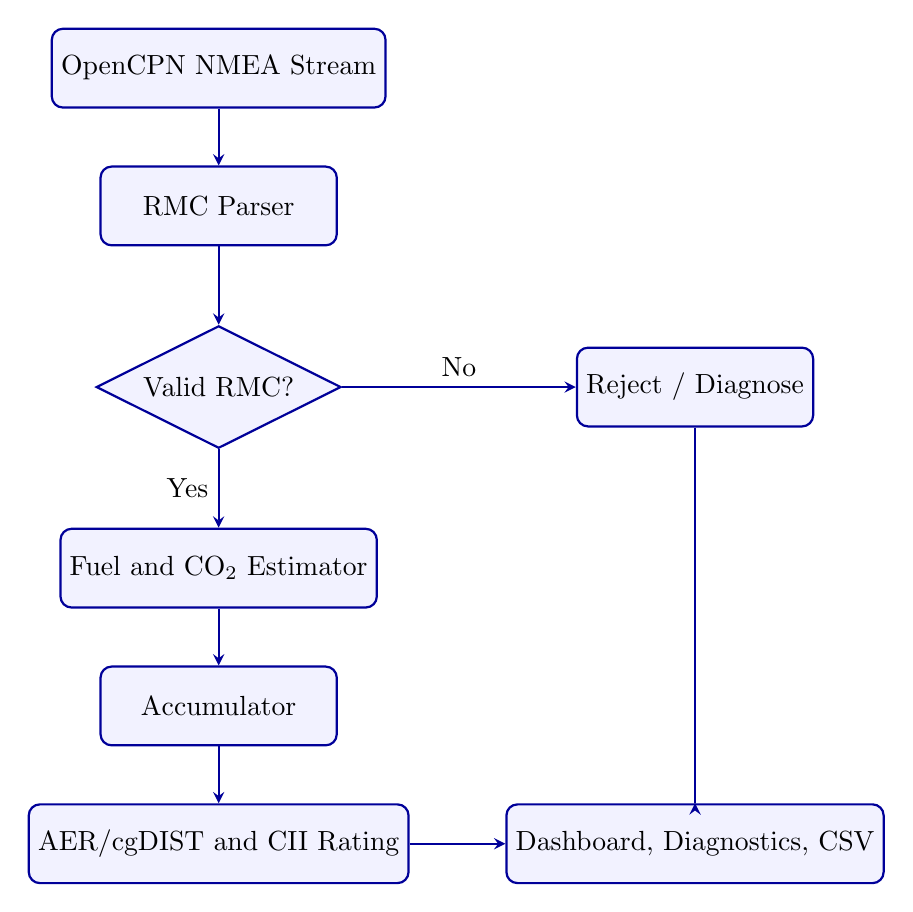
\begin{tikzpicture}[node distance=1.75cm]
    \node (start) [startstop] {OpenCPN NMEA Stream};
    \node (parser) [process, below of=start] {RMC Parser};
    \node (valid) [decision, below of=parser, yshift=-0.55cm] {Valid RMC?};
    \node (fuel) [process, below of=valid, yshift=-0.55cm] {Fuel and CO$_2$ Estimator};
    \node (accum) [process, below of=fuel] {Accumulator};
    \node (cii) [process, below of=accum] {AER/cgDIST and CII Rating};
    \node (ui) [startstop, right of=cii, xshift=4.3cm] {Dashboard, Diagnostics, CSV};
    \node (drop) [startstop, right of=valid, xshift=4.3cm] {Reject / Diagnose};

    \draw [arrow] (start) -- (parser);
    \draw [arrow] (parser) -- (valid);
    \draw [arrow] (valid) -- node[anchor=east] {Yes} (fuel);
    \draw [arrow] (valid) -- node[anchor=south] {No} (drop);
    \draw [arrow] (fuel) -- (accum);
    \draw [arrow] (accum) -- (cii);
    \draw [arrow] (cii) -- (ui);
    \draw [arrow] (drop.south) |- (ui.north);
\end{tikzpicture}
\caption{Implemented data flow from OpenCPN navigation input to emissions dashboard}
\label{fig:system-architecture}
\end{figure}

The main modules are:
\begin{enumerate}
    \item \textbf{Domain module:} Vessel profile, fuel emission factors, Admiralty fuel estimation, CII reference data, AER/cgDIST computation, and rating classification.
    \item \textbf{Data module:} RMC parsing, checksum validation, Haversine distance calculation, accumulator state, and JSON persistence.
    \item \textbf{Plugin core:} The orchestration layer that receives NMEA sentences, applies filtering and diagnostics, updates accumulated state, and produces dashboard snapshots.
    \item \textbf{OpenCPN adapter:} The plugin class that registers toolbar and NMEA capabilities, loads/saves OpenCPN settings, manages private plugin data files, and connects user actions to the core.
    \item \textbf{User interface and export:} wxWidgets setup dialog, dashboard frame, diagnostics view, annual CSV export, and voyage CSV export.
\end{enumerate}

\section{NMEA Data Processing}
The prototype processes own-ship NMEA 0183 RMC sentences. The parser accepts supported RMC talker IDs and then performs the following checks:
\begin{enumerate}
    \item The sentence must begin with \texttt{\$}, include a checksum delimiter, and contain a valid two-character hexadecimal checksum.
    \item The sentence type must end in \texttt{RMC} and use a supported GNSS talker ID.
    \item The status field must be active rather than void.
    \item Time, date, latitude, longitude, and SOG fields must parse cleanly.
    \item Empty or negative SOG values are rejected.
\end{enumerate}

Within \texttt{PluginCore}, further runtime filtering is applied. The default SOG threshold is 1.0 knot, so port or anchor periods below this threshold are excluded from accumulation. A default SOG outlier limit of 50 knots rejects unrealistic data without changing accumulated totals. Invalid sentence bursts, stale GPS input, processing errors, and year rollover events are recorded as diagnostic events.

\section{Fuel and CO2 Estimation}
For every accepted RMC sentence, the plugin estimates main-engine shaft power using the Admiralty Coefficient model:
\begin{equation}
    P = \frac{\Delta^{2/3} \cdot V^3}{C}
    \label{eq:meth-fuel}
\end{equation}
where $\Delta$ is displacement, $V$ is SOG, and $C$ is the configured Admiralty Coefficient.

The resulting shaft power is converted to fuel rate and CO$_2$ rate:
\begin{equation}
    \dot{m}_f = P \cdot SFOC \cdot 10^{-6}
    \label{eq:meth-fuel-rate}
\end{equation}
\begin{equation}
    \dot{m}_{CO_2} = \dot{m}_f \cdot C_F
    \label{eq:meth-co2-rate}
\end{equation}

The supported fuel conversion factors are implemented for HFO, LFO, MDO, LNG, and methanol. Because the model estimates main-engine fuel use from speed, the dashboard displays operational estimates, not certified fuel-flow measurements.

\section{Distance and Emissions Accumulation}
The first valid fix establishes a baseline and does not accumulate distance. Each subsequent valid and underway fix is compared with the previous fix. The elapsed time is calculated from the RMC date and UTC time, while distance is calculated from latitude and longitude using the Haversine formula:
\begin{equation}
    d = 2r \arcsin\left(\sqrt{\sin^2\left(\frac{\phi_2 - \phi_1}{2}\right) + \cos(\phi_1)\cos(\phi_2)\sin^2\left(\frac{\lambda_2 - \lambda_1}{2}\right)}\right)
    \label{eq:haversine}
\end{equation}
where $\phi$ is latitude, $\lambda$ is longitude, and $r$ is earth radius in nautical miles.

The accumulator adds distance and estimated CO$_2$ only when both the current and previous fixes are eligible for accumulation. This prevents a below-threshold or invalid interval from being bridged as if it were a continuous underway period. The accumulator supports year-to-date state, active voyages, completed voyage records, YTD seed values for mid-year installation, and year rollover archiving.

\section{CII Calculation and Rating}
When accumulated distance is greater than zero, the plugin computes a running AER or cgDIST value:
\begin{equation}
    CII_{attained} = \frac{\text{Total CO}_2 \text{ (tonnes)} \cdot 10^6}{\text{Capacity} \cdot \text{Distance (nm)}}
    \label{eq:meth-running-cii}
\end{equation}

For AER ship types, capacity is DWT. For cgDIST ship types, capacity is GT. The CII reference module stores ship-type coefficients, capacity caps or floors where applicable, rating boundary vectors, and reduction factors for 2023, 2024, 2025, and 2026. Unsupported future years are rejected so that the prototype does not silently invent regulatory values.

\section{Persistence, Export, and User Interface}
Vessel profile settings are stored through OpenCPN's configuration mechanism. Accumulator state is stored as JSON in the plugin-private data directory. This keeps vessel setup and voyage state available across OpenCPN sessions while retaining human-readable state files for debugging.

The wxWidgets setup dialog contains:
\begin{itemize}
    \item a vessel tab for ship name, IMO number, ship type, GT, DWT, Admiralty Coefficient, SFOC, fuel type, and displacement;
    \item an EEXI tab for installed power and reference speed fields, with an operational-awareness disclaimer;
    \item an advanced tab for SOG threshold, target-year override, and YTD seed values.
\end{itemize}

The dashboard displays vessel context, GPS freshness, current SOG, estimated CO$_2$ rate, year-to-date distance and CO$_2$, running AER or cgDIST, required CII, margin to the C/D boundary, current CII rating, active-voyage totals, and the latest diagnostic. CSV export functions create annual summary and voyage breakdown files.

Processing is intentionally synchronous through \texttt{PluginCore}. The parser and calculation path are small enough to run during the OpenCPN NMEA callback, while the dashboard is refreshed through ordinary wxWidgets event handling and timer-based freshness polling. No worker thread is used in this version.

\section{Build and Demonstration Method}
The core/test build is controlled through CMake with \texttt{EEXI\_CII\_BUILD\_TESTS=ON} and \texttt{EEXI\_CII\_BUILD\_OPENCPN\_PLUGIN=OFF}. The OpenCPN plugin wrapper is built separately when wxWidgets and OpenCPN plugin API support are available. The repository also includes a PowerShell UDP demo feed that sends synthetic RMC sentences to \texttt{127.0.0.1:10110}, allowing the plugin dashboard to be demonstrated without physical GPS equipment.

\chapter{Results and Validation}
\label{chap:results}

\section{Introduction}
This chapter reports what has been implemented and verified in the current repository. The validation evidence is limited to automated tests, synthetic replay data, and packaging checks. It does not represent real-vessel fuel validation, class-society approval, or statutory IMO reporting verification.

\section{Implemented Prototype Features}
The current prototype implements the main real-time CII monitoring workflow. Table \ref{tab:implemented-features} summarises the feature status against the actual codebase.

\begin{table}[H]
    \centering
    \small
    \caption{Implemented Feature Status}
    \label{tab:implemented-features}
    \begin{tabularx}{\textwidth}{lXX}
        \toprule
        \textbf{Area} & \textbf{Implemented in Current Repository} & \textbf{Status} \\
        \midrule
        RMC parsing & Checksum validation, active/void status, supported GNSS talkers, position, SOG, date, and time & Complete for RMC workflow \\
        Fuel estimation & Admiralty Coefficient power estimate, SFOC conversion, and fuel-specific CO$_2$ factors & Complete as an estimate \\
        CII calculation & AER/cgDIST, CII reference lines, rating boundaries, and 2023--2026 reduction factors & Complete for modelled ship types and years \\
        Accumulation & Haversine distance, CO$_2$ totals, voyage records, YTD seed, threshold filtering, and year rollover & Implemented and tested \\
        User interface & wxWidgets setup, dashboard, GPS freshness, diagnostics, and toolbar toggle & Implemented in OpenCPN wrapper \\
        Persistence & OpenCPN settings for vessel profile and JSON persistence for accumulator state & Implemented and tested \\
        CSV export & Annual summary CSV and voyage breakdown CSV & Implemented and tested \\
        Packaging & Plugin-manager tarball/XML generation and checksum smoke test & Implemented and tested \\
        EEXI calculator & EEXI context and input fields are present, but no full statutory EEXI pass/fail calculation is implemented & Partial / future work \\
        Regulatory validation & No class-society, DCS, SEEMP, or official EEXI/CII submission validation & Not implemented \\
        \bottomrule
    \end{tabularx}
\end{table}

\section{Automated Test Results}
The CTest suite was run in the current workspace on 9 July 2026. All six CTest entries passed. The suite covers pure domain calculations, CII reference values, NMEA parsing, persistence, accumulator behaviour, replay validation, and packaging metadata.

\begin{table}[H]
    \centering
    \small
    \caption{CTest Validation Summary}
    \label{tab:ctest-summary}
    \begin{tabularx}{\textwidth}{lXX}
        \toprule
        \textbf{CTest Entry} & \textbf{Coverage} & \textbf{Result} \\
        \midrule
        \texttt{eexi\_cii\_domain\_tests} & Fuel emission factors, AER/cgDIST capacity selection, Admiralty fuel estimate, threshold behaviour, invalid profile values & Passed \\
        \texttt{eexi\_cii\_aer\_engine\_tests} & Reduction factors, reference coefficients, capacity caps/floors, required CII, rating boundaries, cgDIST path & Passed \\
        \texttt{eexi\_cii\_data\_tests} & RMC checksum/parsing, Haversine distance, CSV export, settings encoding, JSON/file persistence & Passed \\
        \texttt{eexi\_cii\_accumulator\_tests} & Baseline fix handling, threshold gaps, YTD seed, voyage records, year rollover, PluginCore snapshots and diagnostics & Passed \\
        \texttt{eexi\_cii\_replay\_validation\_tests} & Synthetic RMC replay through the same parser, fuel, accumulator, and AER path used by PluginCore & Passed \\
        \texttt{eexi\_cii\_packaging\_tests} & Plugin-manager tarball generation, metadata XML fields, SHA256 checksum, package layout & Passed \\
        \bottomrule
    \end{tabularx}
\end{table}

\section{Synthetic Replay Validation}
The replay fixture in \texttt{tests/fixtures/replay\_validation\_route.nmea} is a deterministic synthetic RMC track. It contains four valid RMC fixes and three one-hour underway intervals. The validation profile is a bulk carrier with 80,000 tonnes DWT, 50,000 GT, 90,000 tonnes displacement, Admiralty Coefficient 680, SFOC 175 g/kWh, and HFO fuel.

\begin{table}[H]
    \centering
    \caption{Synthetic Replay Fixture Results}
    \label{tab:replay-results}
    \begin{tabularx}{0.86\textwidth}{lX}
        \toprule
        \textbf{Metric} & \textbf{Replay Result} \\
        \midrule
        Valid RMC fixes & 4 \\
        Underway intervals & 3 one-hour intervals \\
        Expected distance & 180.121382199 nautical miles \\
        Expected estimated CO$_2$ & 8.343361800 tonnes \\
        Expected AER & 0.579009672 gCO$_2$/(dwt-nm) \\
        Expected CII rating & A \\
        Actual CTest result & Passed within configured floating-point tolerance \\
        \bottomrule
    \end{tabularx}
\end{table}

This replay proves that the core processing chain is internally consistent for the fixture: RMC parsing, fuel estimation, Haversine distance accumulation, AER computation, and rating classification all produce the expected result. It does not prove real fuel-consumption accuracy because the replay has no measured fuel-flow reference.

\section{Dashboard and Export Behaviour}
The implemented dashboard displays live SOG, estimated CO$_2$ rate, YTD distance, YTD CO$_2$, running AER/cgDIST, required CII, margin to the C/D boundary, and CII rating. It also reports GPS freshness states, including no fix and stale GPS after more than 60 seconds without valid RMC data. Diagnostics are recorded for invalid RMC bursts, outlier rejection, processing errors, settings failures, persistence failures, CSV export outcomes, and year rollover.

The export module has two outputs:
\begin{itemize}
    \item \textbf{Annual CSV summary:} year, ship name, IMO number, ship type, capacity type, capacity, total distance, total CO$_2$, AER/cgDIST, CII rating, and required CII.
    \item \textbf{Voyage CSV breakdown:} voyage name, start/end timestamps, displacement, distance, CO$_2$, AER, and whether the record is named or unassigned.
\end{itemize}

\section{Packaging Outcome}
The repository includes a packaging helper for the initial OpenCPN plugin-manager target \texttt{msvc-wx32} / \texttt{x86}. The packaging smoke test creates a fake plugin DLL, runs the packaging script, verifies the generated tarball and XML metadata, checks the API version and target fields, and confirms that the XML checksum matches the tarball SHA256 hash. This validates packaging mechanics, not runtime behaviour inside OpenCPN.

\section{Validation Boundary}
The most important result is also a limitation: the project is a credible operational-awareness prototype, but it is not a certified compliance product. The automated tests verify the implementation against hand-calculated and deterministic expectations. The synthetic replay verifies the data path under controlled conditions. The field-test gate remains open for fresh install, upgrade, corrupted state, missing GPS, invalid NMEA, SOG outliers, long replay, mid-year seed, year rollover, restart recovery, and CSV export scenarios in a live OpenCPN environment.

\chapter{Conclusion and Future Work}
\label{chap:conclusion}

\section{Conclusion}
This project produced a working OpenCPN plugin prototype for real-time CII operational awareness. The implemented pipeline accepts own-ship NMEA 0183 RMC data, rejects invalid or unsuitable inputs, estimates fuel and CO$_2$ from a configurable vessel profile, accumulates distance and emissions, and displays a running AER or cgDIST value with an A--E CII rating. The work is aligned with the KMOU OceanX International Summer School 2026 theme because it translates maritime decarbonisation regulation into an inspectable open-source software artefact.

The project also clarified an important engineering boundary. Real-time CII awareness can be demonstrated using only navigation data and vessel profile assumptions, but official compliance cannot be inferred from that alone. The current prototype is useful for education, simulation, and operational awareness. It does not replace measured fuel data, statutory reporting, class-society verification, or the full IMO correction-factor framework.

\section{Achievement of Objectives}
\begin{enumerate}
    \item \textbf{Regulatory review:} The report reviewed EEXI and CII requirements and corrected the regulatory references to the current IMO guideline set used by this prototype.
    \item \textbf{CII calculation pipeline:} The prototype implements RMC parsing, Admiralty fuel estimation, CO$_2$ estimation, Haversine distance accumulation, AER/cgDIST calculation, and CII rating classification for the modelled ship types and 2023--2026 reduction factors.
    \item \textbf{OpenCPN integration:} The repository includes an OpenCPN plugin wrapper, toolbar control, setup dialog, dashboard, diagnostics, JSON persistence, and CSV export functionality.
    \item \textbf{Repeatable demonstration:} A synthetic replay fixture and UDP demo feed are present, allowing the project to be demonstrated without real shipboard equipment.
    \item \textbf{Validation:} The current CTest suite passed all six entries, including replay and packaging tests.
\end{enumerate}

\section{Recommendations and Future Work}
\begin{itemize}
    \item \textbf{Complete the simplified EEXI calculator:} Implement attained and required EEXI display with a strong disclaimer that the result is not a statutory substitute.
    \item \textbf{Add direct fuel-flow integration:} Support NMEA 2000 or other fuel-flow data sources so that measured fuel data can replace Admiralty Coefficient estimates where available.
    \item \textbf{Implement CII correction factors:} Add the relevant MEPC.355(78) correction-factor and voyage-adjustment paths, while clearly separating official and estimated values.
    \item \textbf{Run the field-test gate:} Validate installation, upgrade, long replay, missing GPS, corrupted persistence, restart recovery, year rollover, and CSV export inside OpenCPN.
    \item \textbf{Compare against real vessel data:} Use anonymised voyage, noon-report, and fuel-flow records to quantify estimation error under different loading and weather conditions.
    \item \textbf{Improve operational guidance:} Add scenario planning and speed-sensitivity views so operators can see how speed changes affect projected CII.
\end{itemize}

\section{Final Statement}
The project demonstrates that open-source navigation software can host a practical maritime decarbonisation awareness tool. Its strongest contribution is not regulatory certification, but transparency: the formulas, assumptions, source code, tests, and limitations are visible. That makes the prototype suitable for a summer-school project, further research, and future engineering extension.


\bibliographystyle{IEEEtran}
\bibliography{references}

\appendix
\chapter{Appendices}
\label{chap:appendix}

\section{Appendix A: Core Calculation Excerpts}
This appendix includes representative excerpts from the implemented C++ source. The full source remains in the repository under \texttt{src/}.

\subsection{Fuel Estimation}
\begin{lstlisting}[language=C++, caption={Implemented Admiralty Coefficient fuel-estimation function.}, label={lst:fuel-estimator}]
FuelEstimate estimate_fuel(
    const double sog_knots,
    const VesselProfile& profile,
    const double sog_threshold
) {
    if (sog_threshold < 0.0) {
        throw std::invalid_argument("SOG threshold cannot be negative");
    }

    if (sog_knots < sog_threshold) {
        return FuelEstimate{0.0, 0.0, 0.0, true};
    }

    if (profile.displacement <= 0.0) {
        throw std::invalid_argument("Displacement must be greater than zero");
    }

    if (profile.admiralty_coefficient <= 0.0) {
        throw std::invalid_argument("Admiralty Coefficient must be greater than zero");
    }

    if (profile.sfoc < 0.0) {
        throw std::invalid_argument("SFOC cannot be negative");
    }

    const double displacement_term = std::pow(profile.displacement, 2.0 / 3.0);
    const double speed_term = std::pow(sog_knots, 3.0);
    const double shaft_power_kw =
        displacement_term * speed_term / profile.admiralty_coefficient;
    const double fuel_rate_tonnes_hr = shaft_power_kw * profile.sfoc / 1000000.0;
    const double co2_rate_tonnes_hr =
        fuel_rate_tonnes_hr * emission_factor(profile.fuel_type);

    return FuelEstimate{
        shaft_power_kw,
        fuel_rate_tonnes_hr,
        co2_rate_tonnes_hr,
        false
    };
}
\end{lstlisting}

\subsection{AER/cgDIST Calculation}
\begin{lstlisting}[language=C++, caption={Implemented AER/cgDIST calculation and CII rating entry point.}, label={lst:aer-engine}]
AERResult compute_aer(
    const double total_co2_tonnes,
    const double total_distance_nm,
    const VesselProfile& profile,
    const int year
) {
    if (total_co2_tonnes < 0.0) {
        throw std::invalid_argument("Total CO2 cannot be negative");
    }
    if (total_distance_nm <= 0.0) {
        throw std::invalid_argument("Total distance must be greater than zero");
    }

    const double capacity = profile.cii_capacity();
    if (capacity <= 0.0) {
        throw std::invalid_argument("CII capacity must be greater than zero");
    }

    const double attained =
        total_co2_tonnes * 1000000.0 / (capacity * total_distance_nm);
    const double required = required_cii(profile.ship_type, capacity, year);
    const RatingBoundaries boundaries =
        rating_boundaries(profile.ship_type, capacity, year);

    return AERResult{
        attained,
        cii_rating(attained, profile.ship_type, capacity, year),
        required,
        boundaries,
        uses_cgdist(profile.ship_type)
    };
}
\end{lstlisting}

\section{Appendix B: Validation Command}
The repository validation run used the following command from the project root:

\begin{lstlisting}[language=bash, caption={Automated validation command.}, label={lst:ctest-command}]
ctest --test-dir build --output-on-failure
\end{lstlisting}

The run completed with all six CTest entries passing. The entries were domain tests, AER engine tests, data tests, accumulator tests, replay validation tests, and packaging tests.


\end{document}
